Starting from the ligand and the protein receptor structures, IDSite carries out flexible ligand docking with Glide.
The flexible ligand docking protocol generates a large number of ligand conformations that are then docked into the rigid receptor.
The first step in Glide docking is to define the binding box and calculate the receptor grid.
As in Glide, in IDSite the binding site is defined as a box centered at the center of selected residues or a ligand (if the structure contains a ligand).
Because we start from the apo structure of CYP2D6 (PDBID: 2F9Q.
See below for details about the protein preparation), the center of the binding box is selected as the centroid of the residues Glu216, Asp301, Thr309, and Phe483.
The box dimension on each side is set to 10 angstroms for the inner box and 20 angstroms for the outer box.
After the grid generation, IDSite samples the conformations of freely rotatable bonds and rings with Glide Standard Precision (SP).
In order to increase sampling, IDSite uses reduced Van der Waals (VDW) radii and skips the default filtering with a rough score within Glide (also referred to as expanded sampling).
Similar poses are clustered according to their RMSD (cutoff 2.0 angstroms).
Finally, a post-docking minimization is performed and the top 60 minimized poses according to the Glide SP score are retained.
These poses are then screened to remove the poses with obvious steric clashes, with too many atoms outside the inner binding box, or without atoms close to the heme iron (Table 3.1).
The remaining poses are then passed to the first refinement stage.
IDSite uses reduced VDW radii for nonpolar atoms both in the protein receptor and the ligand, so that slight steric clashes are tolerated during the docking stage.
For the protein receptor the VDW scaling factor is fixed at 0.40, while for the ligand, the scaling factor starting from 0.80 is adaptively adjusted until at least 4 valid poses are found.
With highly flexible ligands and relatively high scaling factors, Glide often finds only a handful of valid poses, and even fewer survive after IDSite screening.
However, if the scaling factor is set too low, the docked poses may contain too many serious steric clashes, which can cause problems in the subsequent minimization.
If IDSite fails to find enough valid poses, the scaling factor is adjusted and the number of poses to pass the initial docking phase in Glide is increased accordingly to augment sampling.
Since a typical CYP2D6 substrate forms a highly conserved salt bridge with either Glu216 or Asp301,125 IDSite employs this conserved interaction to reduce the sampling cost of the CYP2D6-docking in the following way: IDSite adds a positional constraint to ensure that the generated poses fulfill at least part of the preferred conserved interactions.
The positional constraint defines a spherical region in the receptor that is within 4.0 angstroms of the center of the Glu216, Asp301, and Ser304 residues (Figure 3.2).
It is required that during docking and post- docking minimization each pose should maintain at least one hydrogen-bond donor inside the spherical region.
If the ligand contains other hydrogen-bond donors except for the basic nitrogen, the constrained docking is likely to generate poses that form hydrogen bonds instead of the salt bridge to Glu216 or Asp301.
However, IDSite is able to distinguish these poses and filter them via an additional salt bridge filter in the pose screening (Table 3.1), so that only the poses with a stable salt bridge are allowed to pass to the refinement stage.

\begin{figure}[h]
\centering
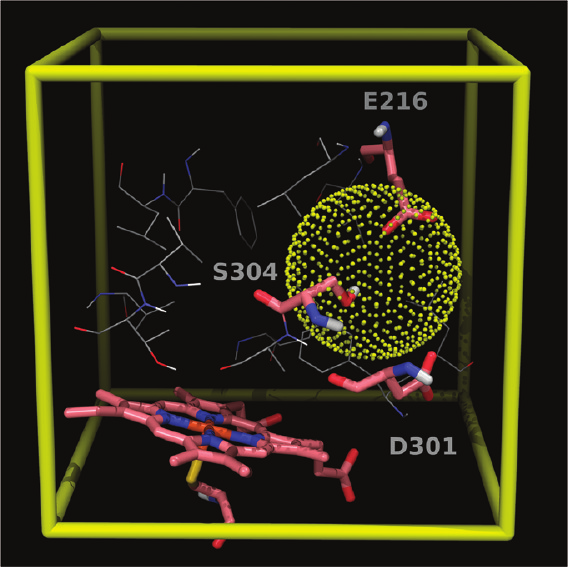
\includegraphics[width=0.35\textwidth]{figures/idsite/glide.png}
\caption{An overview of the entire IDSite procedure.}
\label{fig:idsite_glide}
\end{figure}
